\documentclass[tikz,border=4pt]{standalone}
\usepackage{amsmath}
\begin{document}
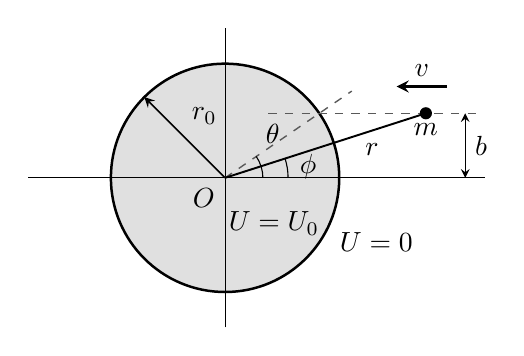
\begin{tikzpicture}[>=stealth, thick, scale=1.0]
  % Shaded potential sphere r <= r0
  \fill[black!12] (0, 0) circle (1.45);
  \draw[line width=0.9pt] (0, 0) circle (1.45);

  % Axes
  \draw[line width=0.4pt] (-2.5, 0) -- (3.3, 0);
  \draw[line width=0.4pt] (0, -1.9) -- (0, 1.9);
  \node[below left] at (0, 0) {$O$};

  % Radius r0 arrow
  \draw[->, line width=0.6pt] (0, 0) -- (135:1.45);
  \node[above right] at (135:0.78) {$r_0$};

  % Incident line at y = b
  \def\bval{0.82}
  % Intersection with circle: angle = asin(0.82/1.45) = 34.4 deg
  \coordinate (P) at (2.55, 0.82);

  % Dashed horizontal path and radial extension at hit point
  \draw[dashed, line width=0.5pt, black!65] (0.55, \bval) -- (3.25, \bval);
  \draw[dashed, line width=0.5pt, black!65] (0, 0) -- (34.4:1.95);

  % Position vector r to particle m
  \draw[line width=0.7pt] (0, 0) -- (P);
  \fill (P) circle (2.2pt) node[below] {$m$};
  \node[below right] at (1.65, 0.56) {$r$};

  % Velocity arrow v
  \draw[->, line width=0.9pt] (2.82, 1.16) -- (2.18, 1.16);
  \node[above] at (2.5, 1.16) {$v$};

  % Impact parameter b
  \draw[<->, line width=0.4pt] (3.05, 0) -- (3.05, \bval) node[midway, right] {$b$};

  % Angles theta (0 to 34.4 deg) and phi (0 to 17.8 deg) with distinct radii
  \draw[line width=0.4pt] (0.80, 0) arc (0:17.8:0.80);
  \node[right] at (0.82, 0.14) {$\phi$};
  \draw[line width=0.4pt] (0.48, 0) arc (0:34.4:0.48);
  \node[above] at (27:0.68) {$\theta$};

  % Potential labels
  \node at (0.62, -0.58) {$U = U_0$};
  \node at (1.92, -0.82) {$U = 0$};
\end{tikzpicture}
\end{document}
